\documentclass[journal,10pt]{IEEEtran}
\usepackage{amsmath,amssymb,amsthm}
\usepackage{booktabs,array,graphicx}
\usepackage{cite}
\usepackage{url}
\usepackage{needspace}
\usepackage[hidelinks]{hyperref}
\newcommand{\E}{\mathbb{E}}
\newcommand{\R}{\mathbb{R}}
\newcommand{\HF}{\mathrm{H}}
\newcommand{\LF}{\mathrm{L}}
\newcommand{\Var}{\operatorname{Var}}
\newcommand{\Cov}{\operatorname{Cov}}
\newcommand{\pending}[1]{\par\noindent\textit{Pending: #1}\par}
\newtheorem{proposition}{Proposition}
\newtheorem{assumption}{Assumption}
\title{Information-Stratified Policy Optimization for Physics-Based Design Automation with Multi-Fidelity Evaluators}
\author{Research working draft}
\markboth{ISPO Research Working Draft, October 12, 2026}{ISPO: Information-Stratified Policy Optimization}
\begin{document}
\maketitle
\begin{abstract}
Physics-based design automation combines natural-language requirements, discrete configuration decisions, and continuous physical parameters. Evaluators can supply objective values, constraint losses, governing-equation residuals, and sensitivities at substantially different costs. We formulate information-stratified policy optimization as the problem of using these signals to post-train a design policy for a specified high-fidelity objective under an evaluation budget. ISPO combines a structured language policy and stochastic numerical head with leave-one-out baselines, component control variates, and corrected multi-fidelity updates. Cheap physics signals form an auxiliary update, while randomized high-fidelity evaluations correct its discrepancy using recorded inclusion probabilities. Residual and adjoint information support objective-aware error estimation and the allocation of additional evaluations. Conditional estimator identities distinguish target consistency from the empirical value of each information type. The experimental protocol isolates estimator accuracy, learning efficiency, and generalization across controlled thermal design, data-center layouts, and aerodynamic design. A seeded controlled study supports residual-informed path updates; full-budget, cross-domain, and generalization experiments remain in progress.
\end{abstract}
\noindent\textbf{Note to Practitioners---}
Engineers often screen many candidate designs with a fast approximation before checking a small number with a detailed simulator. A design generator trained entirely on the fast approximation can learn to favor configurations that appear attractive there but perform poorly under the detailed model. The proposed workflow uses inexpensive evaluations for broad exploration and reserves detailed evaluations for calibration and selected uncertain designs. When a predicted physical field is available, a governing-equation check can help decide which candidates deserve additional evaluation; an objective-specific sensitivity calculation can further improve the screening score. The intended application is repeated design work across changing requirements, rather than replacing engineering sign-off for one installation. Adoption requires a reproducible design compiler, a calibrated detailed evaluator, and an explicit account of all simulation and training costs. Data-center layouts provide the motivating application, with controlled thermal and aerodynamic problems used to study the method. The present draft specifies the workflow and evaluation protocol; evidence of operational savings and design quality will be added after experiments. Every released design must still pass the application-specific physical and geometric checks.
\par
\begin{IEEEkeywords}
Design automation, language-model post-training, multi-fidelity evaluation, physics-based optimization, control variates.
\end{IEEEkeywords}
\Needspace{6\baselineskip}
\section{Introduction}
\IEEEPARstart{P}{hysics}-based design automation must turn requirements into a configuration that can be compiled, simulated, and checked. In a data center, this includes the arrangement and orientation of racks and cooling equipment, its supply/return architecture, and operating parameters. Similar structure appears in aerodynamic and thermal component design: a discrete choice determines the design family, while continuous parameters determine its geometry or operating point. A language model offers a common interface for requirements and structured proposals, and post-training can adapt this interface to repeated design tasks.

The cost of physical feedback is a central constraint. A reduced model or coarse simulation can score many designs, while a detailed simulation may require substantial computation and geometry preparation. Evaluators also differ in the information they expose. A black-box solver returns a score; a diagnostic interface returns component losses; a residual interface checks a proposed field against governing equations; and a differentiable or adjoint interface returns sensitivities. This creates an opportunity to purchase and combine several kinds of feedback instead of treating every evaluator call as an interchangeable scalar reward.

The learning objective is nevertheless defined by a particular high-fidelity evaluator. Directly maximizing a cheap score can favor configurations whose apparent improvement comes from model discrepancy. High-fidelity checks after training reveal this discrepancy but do not themselves determine how earlier updates should have used cheap information. Conversely, evaluating every sampled design at high fidelity may leave too few updates to learn a reusable policy. The relevant question is how available physical information can reduce the cost of learning toward the specified target.

We propose \emph{information-stratified policy optimization} (ISPO), a post-training framework that jointly manages physical fidelity, information content, and update cost. It uses cheap physical signals to predict a target-consistent update, then corrects the prediction with a randomized subset of high-fidelity evaluations. Recording the sampling probabilities allows objective-aware selection without silently changing the training distribution. Continuous sensitivities enter through a numerical output head; discrete structure remains an explicit stochastic decision.

The paper develops three connected claims: physical information can improve the economy of target-directed post-training; objective-aware residuals can support reliable learning with imperfect approximations; and the resulting policy can reuse physical design knowledge across requirements. ISPO addresses these claims through information-aware control variates, residual-guided acquisition, and distinct update routes for structural and numerical decisions. Its conditions for target consistency are stated explicitly. Each claim has a corresponding experiment: information and cost ablations test learning economy, fidelity-gap studies test the role of residuals, and non-language-policy, search, and held-out design comparisons test the value of reusable post-training. The complete experimental program is retained as the evidence needed to establish these claims.

Data-center design is the motivating application. A controlled thermal benchmark provides inexpensive reference evaluations and tunable approximation errors; an aerodynamic benchmark supplies an additional problem with a mature adjoint interface. This organization makes the method testable before undertaking large layout experiments, while keeping the intended contribution in post-training for physical design automation.

\section{Related Work}
\subsection{Verifiable and Differentiable Physical Feedback}
RLVP post-trains language models to generate PDE solver code using continuous solution-accuracy and residual-consistency rewards~\cite{cai2026rlvp}. Its residual diagnostic scores the generated solution against a reference-based verifier. ISPO studies structured designs and the discrepancy between cheap and target evaluations; the proposed residual signal is evaluated on a cheaply obtained field for the same design.

PIRF fine-tunes diffusion models through differentiable physical rewards~\cite{yuan2025pirf}. GRADE propagates reward gradients through relaxed language-model generation~\cite{nel2025grade}. GRADE's shared-vocabulary reward interface differs from an external physical solver that consumes parsed numerical parameters. The numerical-head bridge considered here addresses this interface difference. Direct physical backpropagation and continuous physics rewards are established ingredients; their usefulness under heterogeneous evaluation cost is the subject of this study.

GI-PPO adaptively incorporates analytical gradients into policy optimization~\cite{son2023gippo}. HPO explicitly combines score-function and pathwise gradients for hybrid discrete--continuous action spaces~\cite{alvo2026hpo}. These works motivate matched gradient-only and mixed-gradient comparisons. ISPO adds a target evaluator whose feedback may be expensive or partially exposed, requiring a correction and allocation rule across evaluation interfaces.

\subsection{Multi-Fidelity and Gradient Control Variates}
MFPG constructs policy-gradient control variates from correlated low- and high-fidelity samples~\cite{liu2025mfpg}. The October 1, 2026 MFPG-PPO extension addresses correlation loss and variance inflation in modern actor--critic training and includes budget-aware allocation~\cite{liu2026mfpgppo}. It is the principal multi-fidelity baseline. MFPG-PPO explicitly studies the correlation--bias tradeoff caused by re-synchronizing low-fidelity rollouts, and its allocation analysis targets an idealized scalar-surrogate variance. The present information-selection study separately measures parameter-gradient variability and the cost of physical information interfaces. The present problem evaluates the same design at both fidelities, so coupling does not require maintaining matched physical trajectories. The proposed distinction is the use of objective-aware residual and sensitivity signals inside the auxiliary update and acquisition rule.

REBAR and RELAX combine score-function estimation with differentiable control variates for discrete or black-box objectives~\cite{tucker2017rebar,grathwohl2018relax}. Q-Prop combines an analytical critic-based term with a Monte Carlo correction~\cite{gu2017qprop}. These precedents establish the broader idea of using differentiable auxiliary information without optimizing the auxiliary objective alone. The conditional correction below is presented as a candidate construction for the physical design setting, rather than as a new general control-variate identity.


RLOO provides a sequence-level leave-one-out policy-gradient baseline~\cite{ahmadian2024rloo}. ABC revisits learned advantage/value control variates for RLVR~\cite{pan2026abc}, and ABC-Align already studies prediction-powered LLM post-training with adaptive bias control~\cite{frankel2026abcalign}. PPI++ and active statistical inference supply related prediction/correction and acquisition principles~\cite{angelopoulos2024ppipp,zrnic2024active}. These works motivate direct learned-feedback and nonphysical-uncertainty baselines. ISPO's proposed distinction is the physical information available from evaluator states, residuals and adjoints, combined with matched hard designs and complete information cost accounting.

\subsection{Residual-Based Objective Error Estimation}
Adjoint-weighted residual correction is a classical technique for estimating output functionals from approximate PDE states~\cite{pierce2000adjoint}. Wang and Hu already place dual-weighted-residual mesh adaptation and functional calculation inside an RL airfoil-design evaluator~\cite{wang2024mechanism}. Their solver workflow includes fine-mesh solution steps. The present question is whether partly purchased physical information can improve post-training updates and evaluation allocation without requiring a full target solve for every design.

NeuroForge studies residual-based trust for neural CFD surrogates and distinguishes error detection from state correction~\cite{jabbary2026neuroforge}. This distinction is important here: a residual is calibrated against target objective error before it controls acquisition. Raw residual magnitude is not assumed to be a universal certificate for physical quality. The prospective contribution is a coherent and physically grounded combination of target correction, physical error information, and cost-aware post-training, with each numerical and learning ingredient attributed to prior work.


\subsection{Language-Guided Design and Digital Twins}
ChatTwin automates data-center digital-twin scene descriptions through a conversational language interface~\cite{li2023chattwin}. Phythesis combines language-driven layout proposals with physics-guided evolutionary refinement for simulation-ready data-center scenes~\cite{li2025phythesis}. These works establish the design application and motivate a named inference-time comparison. ISPO asks how the proposal policy itself can be post-trained using a corrected allocation of heterogeneous physical feedback across tasks.

Scientific Generative Agent uses language-model proposals for discrete scientific structure and differentiable simulations for continuous optimization~\cite{ma2024sga}. This is a close precedent for the discrete--continuous division of work. The post-training question concerns parameter updates to a reusable proposal policy and their fidelity/cost accounting. The aerodynamic protocol uses an established adjoint framework such as DAFoam~\cite{he2020dafoam}; solver development and conversational simulation tooling are attributed to their own contributions.

\section{Problem Formulation}
\subsection{Tasks, Policies, and Compilable Designs}
A task $p$ specifies requirements, geometry, component inventories, and operating conditions. Inventories are fixed per task so that capacity changes cannot improve the cooling score by changing its denominator. A policy generates a design $d=(s,x)$, where $s$ is a discrete structured configuration and $x\in\R^{m(s)}$ contains continuous parameters. We use the factorization
\begin{equation}
\pi_\theta(d\mid p)=\pi_\theta^{s}(s\mid p)\pi_\theta^{x}(x\mid s,p).
\label{eq:policy}
\end{equation}
The first factor is a grammar-constrained language policy. The second is a bounded stochastic numerical head with an evaluable density and a reparameterization $x=h_\theta(s,p,\epsilon)$. A deterministic compiler maps $d$ into a simulation input. Compiler acceptance establishes schema validity; geometric, boundary-condition, and physical validity are checked separately.

For the data-center application, a hard candidate is a genuine schema-compatible \texttt{.cfdproj} copy. It is evaluated through the engineering compiler and physical simulation chain. A soft vector, relaxed graph, or empty project is not an interchangeable hard candidate. Differentiation acts on numerical parameters of the compiled model or an explicitly defined smooth surrogate. Neither JSON parsing nor the production compiler is assumed differentiable.

\subsection{Target and Evaluation Interfaces}
The reference objective is
\begin{equation}
J_\HF(\theta)=\E_{p\sim\mathcal P}\E_{d\sim\pi_\theta(\cdot\mid p)}[R_\HF(d;p)].
\label{eq:target}
\end{equation}
The reward aggregates declared physical objectives and constraints with fixed scales. In the current data-center specification, total design-condition PUE is the primary objective; lower server exhaust temperature or greater thermal margin is a secondary objective, with inlet and exhaust upper bounds treated as hard constraints. For mixed-cooling tasks, the specification separately defines air, solid and coolant limits using the quantities represented by the solver. Annual PUE and the design-condition cooling contribution are distinguished. The evaluation protocol also reports these quantities separately, including performance among feasible designs. Invalid proposals and solver failures have explicit statuses and a predeclared finite training reward; numerical failure is not silently converted into a successful cheap evaluation.

An evaluator $f$ returns any supported subset of the following signals: $I_0$, a scalar objective or reward; $I_1$, component-wise objective and constraint losses; $I_2$, a governing-equation residual evaluated on a supplied state; and $I_3$, objective sensitivities with respect to declared continuous parameters. An interface record identifies fidelity, state variables, mesh, boundary conditions, closure model, units, supported derivatives, validity status, and measured cost. Availability of $I_3$ does not imply availability of a full state or $I_2$.

For a high-fidelity discrete operator $F_\HF(u;d)=0$ and a lifted cheap state $\tilde u$, the residual signal is
\begin{equation}
r_\HF(d)=F_\HF(\tilde u;d).
\label{eq:residual}
\end{equation}
The operator includes the specified boundaries, source terms, and closures. State lifting, geometry preparation, and operator evaluation are part of the residual cost. A zonal model that supplies only averages does not automatically satisfy this field-level contract.

\subsection{Budgets and Evaluation Distribution}
Total cost includes proposal generation, simulation preparation, forward solves, residual evaluations, adjoints, surrogate training, and policy optimization. We report wall time together with CPU/GPU time and an equivalent target-evaluation budget calibrated from measured calls. Final designs from every method are scored with the same held-out high-fidelity protocol.

The primary setting is a contextual design decision: one complete design is sent to all relevant evaluators. Sequential refinement is an additional deployment protocol. A training batch is sampled from a frozen policy version. The earliest implementation waits for its selected target evaluations before updating; asynchronous execution must retain policy identity and apply a declared staleness or importance-weighting rule.

\subsection{Hypotheses}
The protocol tests three linked hypotheses: objective-aware residual information predicts target discrepancies on the evolving policy distribution; including sensitivities in a corrected auxiliary update improves useful gradient information per unit cost; and post-training amortizes design work across held-out requirements and geometries. No hypothesis is treated as an established result in this draft.

\section{Information-Stratified Policy Optimization}
\subsection{On-Policy Target and RLOO Baselines}
The reference update estimates the gradient of~\eqref{eq:target}, with regularization handled separately. Write $S_\theta(d,p)=\nabla_\theta\log\pi_\theta(d\mid p)$ and
\begin{equation}
Y_\theta(d,p)=(R_\HF(d;p)-b(p))S_\theta(d,p).
\label{eq:reference-gradient}
\end{equation}
The sequence score sums the actual constrained token log-probabilities and the numerical-head log-density, without action-dependent length normalization. Latent numerical draws, their density/Jacobian, and compiled values are preserved when serialization or quantization changes the physical input. A predictable baseline, fitted before the current batch, is independent of its sampled action conditional on the prompt. Under the usual dominated differentiation and finite-moment conditions, $\E[Y_\theta]=\nabla J_\HF$. All paired and cheap-only samples in an update use the same frozen behavior policy and evaluator definitions.

The production backbone is REINFORCE leave-one-out (RLOO)~\cite{ahmadian2024rloo}. For $K\ge2$ independent designs for a prompt, the complete-feedback baseline is
\begin{equation}
b_{-i}=\frac{1}{K-1}\sum_{j\ne i}R_{\HF,j}.
\label{eq:rloo-peer}
\end{equation}
Excluding the design's own reward makes the subtraction unbiased. With randomized target acquisitions $Z_j$ and recorded probabilities $q_j$, a candidate peer baseline is
\begin{equation}
\widehat b_{-i}^{\rm HT}=\frac{1}{K-1}\sum_{j\ne i}\frac{Z_j R_{\HF,j}}{q_j}.
\label{eq:ht-peer}
\end{equation}
Acquisitions are independent conditional on the sampled designs and prior calibration state. Averaging first over their indicators and then over the other independent designs gives $\E[\widehat b_{-i}^{\rm HT}\mid d_i,p]=\E[R_\HF\mid p]$. This provides a first-moment justification for the peer subtraction. The fixed denominator $K-1$ remains defined when no peer is selected. A raw average over an adaptively selected high-fidelity subset does not have this identity.

Current-group RLOO introduces dependence between sample updates. The independent-sample covariance formulas below therefore use predictable baselines, or independently sampled complete prompt-group aggregates as their statistical units. RLOO configurations are audited with repeated independent groups; their variance is not obtained by substituting dependent rollouts into an IID formula.

One on-policy update is taken per collected batch. Group sample-standard-deviation normalization, clipping, and batch reuse are distinct comparison variants~\cite{schulman2017ppo,shao2024deepseekmath}; their update is not claimed to be the unbiased gradient in~\eqref{eq:target}. A common predictable scalar normalization can be absorbed into the learning rate. Prompt-specific scaling defines a reweighted task objective and is recorded explicitly. The numerical head has its own reference density for KL regularization; disabling an adapter does not by itself define that density.

\subsection{Component and Residual Control Variates}
For an independently sampled design, let $L_k(d,p)$ be a cheap vector-valued update. Scalar-reward and component-loss instances take the form $v_k S_\theta$ with fixed declared scales and predictable baselines. A residual-feature instance is $w(d,p)L_k(d,p)$, where the gate is calibrated before the batch and evaluated identically for paired and cheap-only samples. Obtaining $w$ on every required sample is charged to the budget. An averages-only L0 model has no field residual; field-level features require a field-producing L1 evaluator and the target operator.

For $n$ target evaluations in an IID collection of $N\ge n$ designs, with cheap updates obtained on all $N$, the nested estimator is
\begin{equation}
\widehat g_\beta=\overline Y_H-\sum_{k=1}^{M}\beta_k(\overline L_{k,H}-\overline L_{k,N}).
\label{eq:nested}
\end{equation}
The paired subset is uniform and independent of design values. Coefficients are fixed from prior or cross-fitted data. The subtraction is zero-mean, including when $L_k$ is an approximate pathwise or straight-through vector: correctness follows from matched distributions and the correction, not from the auxiliary vector's being a correct physical gradient. Uncorrected straight-through updates remain a separate biased variant.

Define $v=\operatorname{tr}\Cov(Y)$, $A_{jk}=\operatorname{tr}\Cov(L_j,L_k)$, and $b_k=\operatorname{tr}\Cov(Y,L_k)$, conditional on the frozen calibration state. For $v>0$ and nonsingular $A$, let $\beta^*=A^{-1}b$ and $R^2=b^TA^{-1}b/v$; a pseudoinverse gives the corresponding projection for singular $A$. A zero-variance reference is handled separately without dividing by $v$.
\begin{proposition}[Nested multi-component variance]
With finite second moments, predictable coefficients, and the nesting in~\eqref{eq:nested},
\begin{align}
\operatorname{tr}\Cov(\widehat g_\beta)
 &=\frac{v}{n}+\left(\frac1n-\frac1N\right)
    (\beta^TA\beta-2\beta^Tb),\label{eq:variance-general}\\
\operatorname{tr}\Cov(\widehat g_{\beta^*})
 &=\frac{v}{n}\left[1-R^2\left(1-\frac nN\right)\right].
\label{eq:variance}
\end{align}
\end{proposition}
\begin{proof}
The covariance of each nested difference is its population covariance multiplied by $1/n-1/N$. Its cross-covariance with $\overline Y_H$ has the same multiplier. Expanding the covariance trace gives~\eqref{eq:variance-general}; completing the quadratic gives~\eqref{eq:variance}.
\end{proof}

For shared scores, the exact cross term is
\begin{equation}
b_k=\E[u v_k\|S_\theta\|^2]-\langle\E[uS_\theta],\E[v_kS_\theta]\rangle.
\end{equation}
Thus, score-norm-weighted regression is a useful implementation route, but an uncentered moment is not generally the centered gradient covariance. Coefficients are fit with ridge regularization and independent calibration. Their estimation error adds the quadratic term $(1/n-1/N)(\beta-\beta^*)^TA(\beta-\beta^*)$. Predictability preserves the mean; it does not alone guarantee variance reduction. Population-optimal additional columns cannot worsen this fixed-sample variance because their coefficients may be zero. End-to-end efficiency also depends on their acquisition and fitting costs. No universal finite-sample regression inflation factor is assumed.

I1 retains the full declared objective. Component losses may enter the controls, or a token baseline depending only on that token's prefix. Assigning a rack's local temperature loss to its own tokens would discard physical interactions and is not an unbiased credit rule. The prefix-baseline identity subtracts expected return without replacing the global return by a local component.

\subsection{Continuous-Head LAX Route}
Continuous values are sampled after the structural prefix is complete, without feeding them into later stochastic token decisions. Split the joint score into $S_s=\nabla_\theta\log\pi^s_\theta(s\mid p)$ and $S_x=\nabla_\theta\log\pi^x_\theta(x\mid s,p)$. For a fixed differentiable cheap reward $R_\LF$ and an exact conditional reparameterization, define
\begin{equation}
P_\LF=\left(\frac{\partial x}{\partial\theta}\right)^T\nabla_x R_\LF,
\qquad C_\LF=R_\LF S_x.
\label{eq:pathwise}
\end{equation}
Differentiation under the conditional expectation gives $\E[P_\LF-C_\LF\mid s,p]=0$.
When only part of the numerical design has a verified derivative, write $x=(g,u)$, where $g$ contains conditioning geometry and $u$ contains differentiable controls. Apply the same identity conditional on $(s,g,p)$, using $P_\LF^u=(\partial u/\partial\theta)^T\nabla_u R_\LF$ and the conditional control score $S_u$. The conditioning sample $g$ is detached within this auxiliary path. Target score-function terms still cover all geometry and control decisions, while the LF score subtraction covers only $S_u$. Zero-filling an unavailable geometry derivative and subtracting the full numerical score would not implement this identity.
 A LAX-style update~\cite{grathwohl2018relax} is
\begin{equation}
\widehat g_{\rm LAX}
 =\overline{R_\HF S_s}_H
  +\overline{(R_\HF-aR_\LF)S_x}_H+a\overline P_{\LF,N},
\label{eq:lax}
\end{equation}
for a predictable coefficient $a$. It estimates the full gradient, including shared LoRA parameters, when all terms use the same current policy and the structural conditioning is handled as specified. If numerical outputs alter subsequent token probabilities, the additional computation-graph terms must be retained~\cite{alvo2026hpo}.

LAX requires the path derivative and the subtracted score-function reward to be the same function. A consistent soft-geometry proxy or fixed-iteration differentiable solver can satisfy the identity even when it is physically approximate. Using a soft objective for the path term and a different hard objective for the score term cannot. An implicit derivative at an unconverged state also needs validation against the implemented forward function. Approximate sensitivities can always be used as matched auxiliary vectors in~\eqref{eq:nested} or~\eqref{eq:corrected}, without asserting the LAX identity. State-dependent coefficient gates require derivatives of the complete gated proxy in the LAX route.

When target sensitivities are available, a conditional hybrid score/path reference is an additional high-fidelity configuration. A deterministic numerical head requires such a path reference and cannot use a black-box continuous score. Numerical noise scales, action densities, and reference KL are recorded. As Gaussian exploration contracts, score variance may grow; the useful cost reduction of LAX is measured rather than predetermined to concern only one fidelity.

\subsection{Randomized Target Acquisition and AIPW}
For an available cheap-information vector $\mathcal I_i$, predict a target update $\psi_i$, for example a calibrated combination of component and residual controls. Choose $q_i\in[q_{\min},1]$ before seeing the target output, draw independent $Z_i\sim\mathrm{Bernoulli}(q_i)$ conditional on the designs, and use
\begin{equation}
\widehat g=\frac1N\sum_i\left[\psi_i+\frac{Z_i}{q_i}(Y_i-\psi_i)\right].
\label{eq:corrected}
\end{equation}
This augmented inverse-probability correction follows standard inclusion weighting and active inference~\cite{horvitz1952sampling,zrnic2024active}. A fixed-count acquisition scheme needs its actual inclusion probabilities, not a Poisson formula copied after top-$n$ selection.
\begin{proposition}[Conditional correction]
If the reference update has the target expectation, $\psi,q$ are fitted independently of current target outcomes, $\E[Z_i\mid d_i,\psi_i,q_i,Y_i]=q_i>0$, and the first moment is finite, then $\E[\widehat g]=\nabla J_\HF$.
\end{proposition}
\begin{proof}
Conditional expectation of the bracket is $\psi_i+Y_i-\psi_i=Y_i$; taking the outer expectation yields the result. The reference baseline is predictable;~\eqref{eq:ht-peer} provides a separate peer-baseline first-moment extension under independent acquisitions.
\end{proof}

For predictable baselines and independently sampled designs, let $e=Y-\psi$. Conditional independence of the acquisition draws yields
\begin{equation}
\Cov(\widehat g)=\frac1N\Cov(Y)+\frac1N\E[(q^{-1}-1)ee^T].
\label{eq:aipw-variance}
\end{equation}
The reference gradient's own variability and the selection penalty are distinct. A zero-mean LAX adjustment $D=a(P_\LF-C_\LF)$ may be added to the cheap part of~\eqref{eq:corrected}; its expectation is unchanged and the first covariance term becomes $\Cov(Y+D)/N$. The selection term remains determined by $Y-\psi$.

The auxiliary \emph{value} for target acquisition need not be the function used for the path control. Let $H,L,A$ denote target, differentiable cheap and goal-corrected cheap rewards after subtracting the same known analytic component. For independently predictable $\beta,\alpha$, use
\begin{equation}
\widehat H_i=\beta A_i+\frac{Z_i}{q_i}(H_i-\beta A_i),
\qquad D_i=\alpha(P_{L,i}-L_iS_{x,i}).
\label{eq:value-path-separated}
\end{equation}
The augmented score estimates the target reward score, while $D_i$ is zero-mean under the conditional path identity. No derivative of $A$ is required: a residual-corrected value can guide acquisition even when only the original cheap derivative is verified. Known analytic reward terms retain their common score/path treatment outside acquisitions.

For an IID RLOO group of size $K$, define $T_i=(S_i-\overline S)/(K-1)$ with the \emph{joint} structural/numerical score and let $G_H$ be its complete target update. Complete augmented peers give
\begin{equation}
G=G_H+\alpha C_L+\sum_i(Z_i/q_i-1)(H_i-\beta A_i)T_i,
\label{eq:group-value-path}
\end{equation}
where $C_L=\overline P_L-\sum_i L_i(S_{x,i}-\overline S_x)/(K-1)$. Conditional on the realized group, the mean is $G_H+\alpha C_L$ and the acquisition-variance trace is $\sum_i(q_i^{-1}-1)(H_i-\beta A_i)^2\|T_i\|^2$. At fixed $\beta$, changing $\alpha$ changes the proposal-group control while leaving conditional purchase noise unchanged. The law of total covariance separates these sources across independent groups, without treating within-group updates as independent.

Minimizing the trace of the selection term for a feasible expected acquisition budget gives the oracle rule
\begin{equation}
q^*(\mathcal I)=\operatorname{clip}_{[q_{\min},1]}
\sqrt{\frac{\E[\|e\|^2\mid\mathcal I]}{\eta h(\mathcal I)}}.
\label{eq:allocation}
\end{equation}
Here $h$ is incremental target cost and $\eta$ enforces the expected budget. The required quantity is conditional squared update error, not only residual size or mean absolute reward error. For score-only controls, the design's score norm enters this quantity. An uncertainty-only predictor is a matched baseline for residual-assisted acquisition.

Defensive mixing with a uniform probability $q_0$ gives $q_D\ge\alpha q_0$ and hence $\E[\|e\|^2/q_D]\le\alpha^{-1}\E[\|e\|^2/q_0]$. This bounds a weighted second moment, not the total variance by the same factor in every distribution. Estimated uncertainty, gradient-norm approximations, and weighted calibration are audited. Hard resource limits and zero-target batches require an explicit stopping protocol; a retrospective selection change invalidates the recorded propensity.

\subsection{Discrete Structures and Physical Residuals}
Small structural decisions are conditionally enumerated in the cheap model using the current policy probabilities. Rao--Blackwellization integrates the declared random variable while retaining the correct conditional distribution of descendants, including the numerical head. It provides a cheap conditional expectation, not the high-fidelity gradient by itself. General discrete structures may use a RELAX estimator with its required conditional relaxed sample~\cite{grathwohl2018relax}. Exact enumeration, RELAX, ordinary score estimation, and an uncorrected straight-through diagnostic are individually identified and costed.

For a smooth objective $Q$, a cheap state and an approximate adjoint define
\begin{align}
F_{\HF,u}(\tilde u;d)^T\hat\lambda&\approx Q_u(\tilde u,d)^T,\\
\widetilde Q(d)&=Q(\tilde u,d)-\hat\lambda^TF_\HF(\tilde u;d).
\label{eq:dwr}
\end{align}
This uses classical output-error correction~\cite{pierce2000adjoint,wang2024mechanism}. The target operator includes boundary conditions and closures. Energy-only residuals, mapped fields, and surrogate turbulence estimates are named interfaces with correspondingly restricted calibration. A single normalized solver residual is not a complete residual vector for an adjoint product.
\begin{assumption}[Local residual-to-output model]
The target solution is locally unique; $F_\HF,Q$ have bounded second derivatives; the inverse Jacobian is bounded near the selected branch; and the cheap state is sufficiently close to it. The residual uses the same complete target operator and boundaries. Let $\lambda$ be the exact adjoint at the cheap state and suppose its approximation error is bounded in the dual norm.
\end{assumption}
Taylor expansion gives
\begin{equation}
|Q(u_\HF,d)-\widetilde Q(d)|
 \le C_1\|r_\HF\|^2+C_2\|\lambda-\hat\lambda\|\|r_\HF\|.
\label{eq:local-bound}
\end{equation}
Indeed, the state error is $-F_u^{-1}r+O(\|r\|^2)$ locally; inserting it into the objective expansion cancels the linear error with the exact adjoint. The approximate adjoint leaves the stated dual-norm product. Geometry preparation, lifting, closure recovery, and adjoint cost are all charged. The value relation is not a derivative-error bound; differentiating a corrected objective needs its own directional checks.

\subsection{Two Explicit Feedback Regimes}
The \emph{target-corrected regime} retains every correction in~\eqref{eq:nested}, \eqref{eq:lax}, or~\eqref{eq:corrected}. Physical information changes variance and acquisition, while the defined mean target is unchanged. A very small positive target probability can still give an unbiased estimator; it may have impractically large uncertainty. There is no universal mathematical minimum target budget. A chosen propensity floor, calibration size, or variance tolerance defines an operational feasibility boundary.

The \emph{trusted-proxy regime} explicitly substitutes a corrected cheap reward in a calibrated region. If $T(d)$ marks that region and the remaining region uses the target reward, define $R_T=T\widetilde R+(1-T)R_\HF$. Suppose $|\widetilde R-R_\HF|\le\epsilon(d)$ on that region. For score-function training,
\begin{equation}
\|\nabla J_T-\nabla J_\HF\|
 \le\E[T\epsilon(d)\|S_\theta\|].
\label{eq:trust-bias}
\end{equation}
This follows directly by subtracting the reward-score expectations. A Lipschitz reward map transfers~\eqref{eq:local-bound} to $\epsilon$; threshold feasibility rewards also require a verified margin from the constraint boundary. Partial residuals do not supply the complete-operator guarantee, and a value bound alone does not justify trusted path gradients. If the complement is rejected or abstained from instead of target-evaluated, the changed deployment/support objective is specified separately.

Low/high score-discrepancy diagnostics are reported in both regimes. The test of proxy exploitation focuses on biased substitution, using discrepancies concentrated where the trained policy goes. Corrected estimators are not claimed to guarantee finite-sample learning quality or fidelity of the target simulator itself; E8 separately checks the latter.

\subsection{Complete Cost and Safe Model Management}
For a fixed information bundle, let $g$ be proposal and shared optimization cost, $\ell$ the cheap-specific evaluation and auxiliary cost, and $h$ the incremental target cost. After a separately recorded calibration/setup charge $C_0$, the remaining allocation budget is $C=C_{\rm total}-C_0=N(g+\ell)+nh$. Combining this with~\eqref{eq:variance} gives the interior allocation
\begin{equation}
r^*\equiv\frac Nn=\sqrt{\frac{hR^2}{(g+\ell)(1-R^2)}},\qquad r^*\ge1.
\label{eq:cost-ratio}
\end{equation}
\begin{proposition}[Idealized equal-cost relation]
For population-optimal controls, fixed per-call costs, $0<R^2<1$, feasible interior $r^*$, and negligible integer rounding,
\begin{equation}
V^*_{\rm CV}(C)=\frac vC
\left(\sqrt{h(1-R^2)}+\sqrt{(g+\ell)R^2}\right)^2.
\label{eq:cost-variance}
\end{equation}
An HF-only method with per-design cost $c_F$ has variance $vc_F/C$. Thus the remaining-budget ratio divides the squared bracket by $c_F$; when its shared costs match, $c_F=g+h$. For different setup costs $C_{0,\rm CV}$ and $C_{0,F}$, the full-budget ratio also multiplies by $(C_{\rm total}-C_{0,F})/(C_{\rm total}-C_{0,\rm CV})$.
\end{proposition}
\begin{proof}
The variance is $v(1-R^2)/n+vR^2/N$. Substitute $N=rn$ and $n=C/[h+r(g+\ell)]$, differentiate in $r$, and insert the stationary point. Boundary allocations and the HF-only arm are compared separately.
\end{proof}

This is a specialization of multifidelity model management~\cite{peherstorfer2016optimal,liu2026mfpgppo}, now with declared shared generation and optimization cost. It does not double-count generation for paired designs. A zero coefficient preserves the target but does not recover wasted cheap-evaluation time. The HF-only arm must be available to skip unnecessary interfaces. Oracle selection may choose the better equal-cost arm; a finite estimated coefficient or cost model does not give an unconditional no-worse guarantee. Correlation monitoring and held-out calibration are empirical safeguards.

Failures are terminal outcomes under a fixed retry policy, with their actual attempt costs recorded. Dividing target cost by success rate is appropriate only for a separately declared retry-until-success accounting model; it is not added again when failure outcomes already enter the training reward and call ledger. Three fidelity levels and adaptive information bundles use their actual covariance, nesting, and cost model rather than assuming a two-level ratio applies unchanged. All acquisition and training efficiencies remain experimental questions.

\section{Experimental Protocol}
\subsection{Task Suite and Physical Verification}
The study includes controlled two-dimensional thermal design, a flagship mixed-cooling data-center layout task with supporting air-cooled configurations, and aerodynamic design. The source and closure models, fidelity levels, admissible designs, physical validation, and state-lifting contracts are frozen per scenario. A project schema check or small numerical gate is not evidence that the complete task suite is solved.

The first controlled pilot changes lid speed, heat-boundary location, and lid direction in a coupled Boussinesq cavity, using a version-pinned finite-volume residual and an implicit adjoint. It is a mechanism pilot for continuous and small discrete decisions. The broader controlled task includes varying heat-source and boundary configurations and admissible obstacles; generalization and all-high-fidelity training are separate requirements. Pilot success does not replace this task expansion. Its common analytic mechanical term is handled identically by strong baselines and reported separately from the fidelity-dependent thermal objective, so a separable known term cannot manufacture an apparent information gain. Manufactured-solution checks, conservation, boundary conditions, refinement, directional sensitivities, repeated-solve noise, and branch/initialization dependence are verified before interpreting learning results.

The principal data-center playground is the authored Shinaide mixed-cooling project, with its server inventory, cold plates and CDU. The registered equipment catalog and single-unit-outage requirement lead to a six-ACU research reference derived from this project; the authored four-unit geometry retains its source identity. The research task retains the cold plates and liquid routes while explicitly using the saved server airflows for fan-assisted operation. Figure~\ref{fig:shinaide} shows the six compiled architecture references. Its retained geometry, loads and equipment parameters carry explicit synthetic-input provenance. The coupled evaluation protocol requires an accepted liquid solution and heat-removal record, the corresponding residual room heat supplied to the air solver, and per-device closure $Q_{\rm IT}=Q_{\rm air}+Q_{\rm liquid}$. Air-side, liquid-side and shared-plant electricity are counted once. The initial steady benchmark prescribes cold-plate generation: the two subsystems share a fixed device heat budget, while controls change thermal margins and hydraulic and electrical costs. Thermal limits are attached separately to the air, solid and coolant quantities represented by the models. Pure-air engineering fixtures verify the compiler, boundary conditions and geometry before the full coupled task is accepted.

For the data-center scenario, equipment counts are fixed per task. The policy chooses containment, row direction/layout, compatible supply/return architecture, ACU shape/placement, and continuous supply temperatures, flows, aisle dimensions, and offsets. Mixed-cooling designs additionally expose liquid-side placement, routes and operating controls verified by the engineering compiler. The air-cooled v1 energy specification couples chilled-water reset, chiller efficiency, tower/pump energy and fan heat; both fidelities use the same accounting module. Total design-condition PUE is the primary objective. Air-cooled configurations retain exhaust temperature or thermal margin as a lower-weight secondary objective and server inlet/exhaust constraints; the mixed-cooling specification adds the corresponding solid and coolant limits. Geometry, airflow closure, leakage, coil capacity, dew-point checks, and N+1 behavior belong to the declared task contract. Numerical limits, equipment assumptions and their evidence status are pinned in the task specification before training; synthetic values are distinguished from equipment calibration.

The high-fidelity pipeline is an actual candidate \texttt{.cfdproj} through geometry/mesh export, physical solve, and face-based post-processing. A small headless export witness establishes its own interface only; room generation, containment, supply/return routing, boundary fingerprints, and the selected architecture menu require separate tests. L0 is a differentiable zonal model. L1 is coarse CFD or a field-producing calibrated surrogate; only L1 can supply the field required for target residual evaluation. Complete and energy-only residual interfaces are reported separately.

The aerodynamic protocol uses 16 reference-preserving upper/lower CST perturbations and DAFoam RANS~\cite{he2020dafoam}. Drag is minimized under lift and geometry constraints. Requirements vary Reynolds number, reference geometry and operating conditions; angle of attack is supplied by the task. A differentiable panel model with a declared drag closure and coarse/fine RANS provide distinct information interfaces. Surface mapping, total shape derivatives and grid quality require verification before policy training. The separately recorded native lift and official drag/angle gates are interface history, not results on this new benchmark. A data-center adjoint interface remains a separate study requirement.

Training, calibration, validation, final test, and out-of-distribution sets are separated by physical task and geometry identity. Paraphrases of a task stay in one split. Heuristic SFT teaches the format and legal proposal construction; optimizer-generated high-fidelity reference designs are not silently imported into the common initialization. They are permitted in a separately costed distillation baseline. Every structured baseline receives equivalent requirements and constraints.



\begin{figure*}[t]
\centering
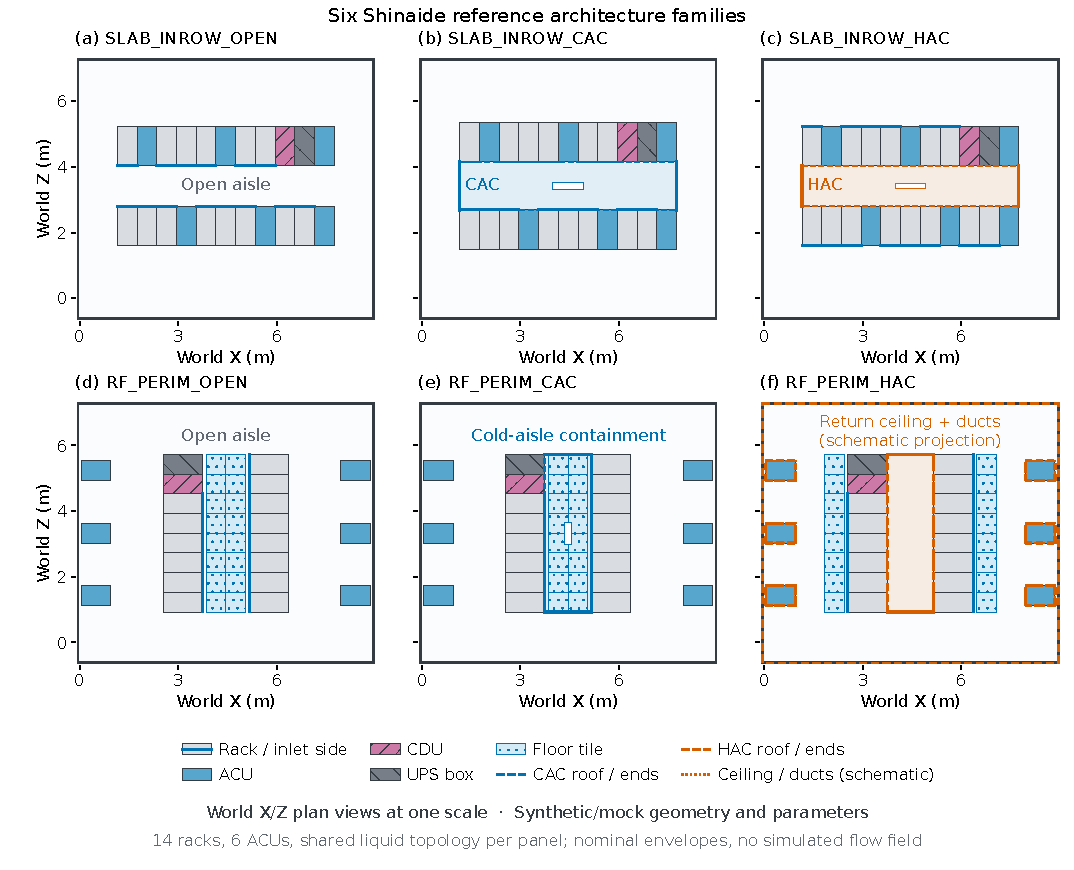
\includegraphics[width=\textwidth]{figures/shinaide_six_family_plans.pdf}
\caption{Six compiled Shinaide architecture references: slab-floor in-row cooling (top) and raised-floor perimeter cooling (bottom), each with open aisles, cold-aisle containment or hot-aisle containment. All panels share the same room coordinates and scale. Equipment envelopes, rack inlet sides, containment sheets and floor tiles come from the saved projects; ceiling returns and vertical ducts are schematic projections. Each reference retains 14 racks, 56 server models, six ACUs and one CDU, with explicit synthetic/mock provenance. These are reference designs, not optimized outcomes or flow fields.}
\label{fig:shinaide}
\end{figure*}

\subsection{E1--E8 Study Matrix}
\textbf{E1: information effects.} A preregistered fractional factorial design studies component controls, residual features, sensitivities, target correction, acquisition, and conditional discrete enumeration. Every cell must correspond to an available interface. The alias matrix and estimable contrasts are recorded so interactions are not inferred from confounded or undefined cells. Scalar-only, pure-HF, pure-L0, and multi-fidelity settings are retained as declared comparison blocks. All policy methods use the numerical head; a digital-token interface comparison is separately isolated.

\textbf{E2: cost--quality frontier.} Sweep target budgets from zero to the all-high-fidelity reference. Zero-target training belongs to the explicit proxy regime, not the corrected estimator. Plot quality and constraint satisfaction against complete CPU/GPU cost and wall time. Controlled tasks supply a tractable all-high-fidelity training reference; it is not assumed to be the global optimum.

\textbf{E3: target information interfaces.} Compare black-box target feedback, surrogate derivatives, residual-only feedback, residual-plus-adjoint output correction, and a validated target adjoint. Complete interface variants are studied where available, with their measured lifting, closure, meshing, and backward costs. The black-box data-center study does not establish its unimplemented adjoint variant.

\textbf{E4: strong method comparisons.} Principal baselines are MFPG-PPO including budget management, faithful nested MFPG/REINFORCE or RLOO, and prediction-powered correction with nonphysical uncertainty~\cite{liu2025mfpg,liu2026mfpgppo,angelopoulos2024ppipp}. HPO, learned differentiable controls, ABC/DAE, and adaptive-bias ABC-Align provide distinct gradient/critic or semi-supervised comparisons~\cite{alvo2026hpo,grathwohl2018relax,pan2026abc,frankel2026abcalign}. Other target-feedback uses include pooling, low-fidelity pretraining followed by target fine-tuning, L0 screening with target-verified self-training, optimizer-to-SFT distillation, on-policy discrepancy-model refresh, and uncertainty penalties. Adaptations preserve each baseline's defining mechanism and receive the same tuning and total evaluation budget.

\textbf{E5: policy and amortization.} Compare a heuristic designer; CMA-ES, multi-fidelity BO, and adjoint descent on the same design parameterization; and an equivalently informed structured neural policy using the same estimator. Report learning/setup cost, deployment cost, task quality, and break-even workload. The need for a language backbone is evaluated across changing and compositional requirements, not inferred from a single task.

\textbf{E6: inference-time agents.} Use the original Qwen policy with the same harness, a named frontier model with a pinned version and equivalent tool/cost budget, Phythesis/SGA-style refinement, and language-generated structure followed by per-task L0 gradient refinement and target validation~\cite{li2025phythesis,ma2024sga}. Common-prompt, common-tools, and common-validation protocols isolate the net benefit of post-training.

\textbf{E7: generalization.} Hold out requirements, geometries, room/equipment scales, equipment placement, architecture combinations, and wording. The 4B and 27B configurations are distinct required study arms, with model hashes and measured numerical-head/adapter memory. Larger-model execution remains under the existing single-GPU authorization; footprint verification is a prerequisite, not evidence of a learning result. Cross-scenario transfer and a joint-scenario policy are reported separately from within-scenario generalization.

\textbf{E8: verification fidelity.} Audit representative final candidates with refined meshes and, where required by flow behavior, transient or repeated-initialization checks. Report changes in feasibility and objective ranking, including computational failures and target-model sensitivity. Optimization of the training evaluator is distinguished from reliability under this additional physical check.

\subsection{Estimator Audit, Regimes, and Ablations}
At preregistered frozen checkpoints, repeated independent batches compare mean error, covariance trace, gradient alignment, and MSE at matched total cost relative to a high-accuracy reference gradient with its own quantified numerical and sampling uncertainty. A finite Monte Carlo reference is not labeled an exact gradient. This is the main mechanism evidence for target consistency and cost allocation. Predictable and HT peer baselines, uniform nesting, multiple controls, and randomized acquisition are tested separately. When RLOO is used, the independent replication unit is a complete prompt group and the audit retains its covariance structure.

The corrected and trusted-proxy regimes are explicitly labeled. A controlled discrepancy concentrated in the policy's frequently visited region probes proxy exploitation. Residual-based acquisition, residual-based substitution, and objective/adjoint correction are separate interventions. A sign-flipped cheap reward is only a sanity check: an adaptive control coefficient can compensate for its sign without demonstrating resistance to realistic policy-distribution shift.

Ablations include scalar versus component controls; residual gates versus residual features; exact versus approximate adjoints; exact versus approximate path derivatives; LAX versus matched auxiliary-vector use; fixed versus calibrated coefficients; uniform, fixed-budget, and randomized objective-aware acquisition; enumeration/RELAX versus score estimation; and numerical heads versus numerical tokens. Direct-path, adaptive-mixing, residual-as-reward, and RLVP-style reward-shape variants isolate the associated ideas~\cite{nel2025grade,son2023gippo,yuan2025pirf,cai2026rlvp}. They are named adaptations or ablations, not purported reproductions on the original output domains.

\subsection{Statistics, Quality, and Complete Costs}
Confirmatory controlled-scene comparisons use at least ten independent training seeds and data-center comparisons at least five. The aerodynamic protocol targets at least five and freezes its final count before training. Pilot runs may be smaller but cannot substitute for these comparisons. Common random numbers couple eligible task evaluations; the estimator's independent replications remain distinct. IQM, paired effect estimates, and hierarchical bootstrap intervals preserve task and seed structure. At most three primary hypotheses are preregistered and receive Holm correction; other analyses are labeled exploratory. These counts are protocol minima, not universal power guarantees.

For the launched controlled study, the fixed-budget analysis uses the latest scheduled checkpoint available at each charged budget, on the common support of all method--seed runs. It does not choose the best observed checkpoint or interpolate unobserved quality. Failed outcomes retain their registered reward and incurred costs. The prepared descriptive intervals resample entire paired training-seed blocks, keeping the two validation tasks fixed; these pointwise intervals do not establish generalization to a task population. This analysis specification was recorded after training launch and before aggregate outcome access, so it is not presented as a pretrial statistical preregistration. Confirmatory tests and any multiplicity correction require a separately frozen hypothesis protocol.

Final task quality uses the same target evaluator. Report feasible completion, constraint violations, hidden-specification satisfaction, and objective quality among feasible designs separately. Server temperatures use declared inlet/exhaust face statistics, rather than unqualified sparse probes. Cooling power, design-condition PUE contributions, RCI/RTI/SHI/RHI, and plant temperatures have pinned definitions. Optimizer search supplies a \emph{best-found, target-verified} reference unless a true bound is certified; signed improvements beyond it are not clipped or recast as impossible.

Full target evaluation is required for displayed accepted design examples and the declared confirmatory test subset. A secondary large-population mean may use a prediction-powered or inclusion-weighted evaluation with randomized target labels~\cite{angelopoulos2024ppipp,zrnic2024active}. That estimate does not imply that every design was physically checked. Applying it to IQM, quantiles, or maxima requires an appropriate functional estimator and its uncertainty, not reuse of a mean formula.

The ledger records generation tokens/time, optimization/backpropagation, calibration, surrogate data/training, compile/export, L0, L1, residuals, adjoints, mesh, solve, post-processing, queueing, retries, and failures. Shared costs are charged once; GPU/CPU conversion is fixed in advance and tested for sensitivity. Cold/warm caches are declared with complete design and boundary fingerprints. Failure cost is recorded on each attempt under the common retry policy. Retrospective success-rate inflation is not added to the same attempt costs.

\subsection{Execution and Completion Evidence}
Every run has an immutable case-local dated logger with code, dependency/evaluator, model, case/project, task-split, seed, configuration, acquisition-probability, cost, checkpoint, and terminal-status identity. A hard candidate is compiled from the recorded agent output, and the evaluated design must match its saved project and solver inputs. Schema-valid artifacts, correct estimator unit tests, physical evaluator gates, short model runs, and confirmatory research experiments are separate evidence levels.

The complete implementation work is tracked as W0--W12: platform repair/security/headless export, task specification, task/prompt generation, DSL/project compiler, energy model, zonal model, target CFD/calibration, metrics/reward, harness, cost ledger, analysis, baselines/reference search, and SFT/RL integration. The residual and adjoint interfaces are additional tracked dependencies. Their acceptance conditions and E1--E8 evidence are maintained in the repository's requirements-to-evidence audit; the study is not complete when only its first physics or software gate passes.

Weak or inconsistent learning first triggers checks of implementation, gradients, physical validity, data/splits, metrics, and budget/tuning fairness. Corrected evidence then determines the supported strengths and operating scope. Reports preserve counterexamples and original failed runs while removing falsified claims. Results enter this manuscript only after independent source-level verification.

\section{Results}
\label{sec:results}
Physical and estimator checks are followed by a seeded controlled learning study. \pending{Full matched-cost comparisons, flagship design benefits and generalization remain to be established; no abandoned historical result is imported.}
\subsection{Seeded Controlled Learning}
Seven fixed-information arms each completed 64 updates for ten paired training seeds from the same legal SFT checkpoint. Evaluation used the two fixed validation tasks at the five declared checkpoints; every attempted outcome was retained. Initial sampled rewards agree across arms within each seed. Figure~\ref{fig:controlled-fixed} reports the terminal paired effects alongside the actual charged cost, without selecting a checkpoint by its reward.

\begin{figure*}[t]
\centering
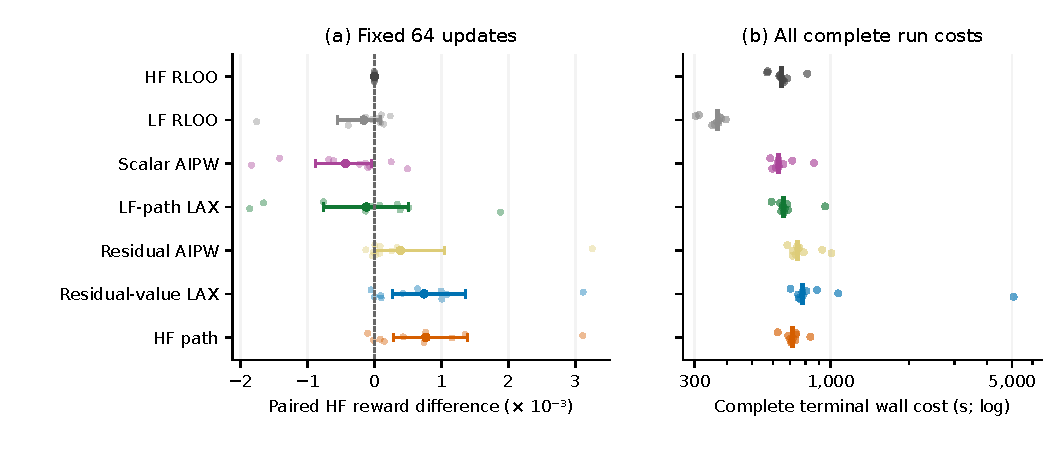
\includegraphics[width=0.98\textwidth]{figures/controlled_fixed_updates.pdf}
\caption{Controlled study at 64 updates, ten paired seeds and two fixed validation tasks. Left: reward difference from HF RLOO; small dots are seed differences, large dots are their means, and bars are descriptive pointwise 95\% paired-seed bootstrap intervals. Right: complete charged wall time for the corresponding runs, including setup, retained failures and target verification; bars indicate medians. This is an update-matched comparison, not a common-wall-budget frontier.}
\label{fig:controlled-fixed}
\end{figure*}

The HF-path and residual-value LAX arms improve the mean terminal target reward relative to HF RLOO in this controlled study. Their paired descriptive intervals lie above zero in Fig.~\ref{fig:controlled-fixed}. The improvement occurs in the thermal component while the analytic control contribution remains close to the reference. These intervals describe variation over the ten training seeds on the fixed tasks; they are not simultaneous tests or evidence of population-level task generalization. The residual-value arm uses a fixed positive acquisition probability and coefficient, and does not test the full adaptive ISPO controller.

The complete information controller has also completed all registered training seeds. Its sampled initial policies agree with the common HF-RLOO start in every seed. At the fixed terminal update, its mean target reward moves positively relative to HF RLOO, primarily through the thermal component; the descriptive paired interval still includes zero. All validation outcomes are retained and independently reconstructed from the original target states. This supports the completed controlled learning experiment while leaving the matched-cost comparison and the full moving-policy information study to be established.

\subsection{Information Value and Cost--Quality Frontier}
For the seven-arm study, the registered strict common-wall-time interval is empty: one recorded model-loading phase exceeds the shortest completed trial. Its delay and all other costs remain in the cohort. Consequently, Fig.~\ref{fig:controlled-fixed} supports the fixed-update comparison only; no cost-frontier advantage is inferred from it. Controlled admission and the complete method comparisons remain necessary for the main efficiency study.
\pending{Matched-budget comparisons; signal costs; randomized acquisition; complete component ablations; broader layout, data-center and aerodynamic validation.}

\subsection{Information Mechanisms}
The controlled finite-volume evaluator supplies a verified physical reference for separating information effects from implementation errors. Directional derivatives, conservation and boundary-response checks establish its declared residual and sensitivity routes. Complete policy-parameter reconstruction supports the corrected value/path assembly. Detailed native-array and interface evidence is retained in the supplementary material.

\subsubsection{Objective-aware residual feedback}
A preregistered set of 60 designs was evaluated at both cavity fidelities, with all attempted outcomes and costs retained. On its 12 predeclared diagnostic anchors, the adjoint-weighted correction was constructed using only the interpolated coarse state and the exact target operator, without a target forward solve or use of target fields. The target scalar was read only after prediction persistence for independent post-validation. Table~\ref{tab:goal-correction} separates the correction's numerical effect from its acquisition cost.
\begin{table}[t]
\centering
\caption{Bounded goal-correction mechanism on 12 predeclared cavity designs. Errors concern the common thermal objective, not field error.}
\label{tab:goal-correction}
\begin{tabular}{lr}
\toprule
Quantity & Measured value \\
\midrule
Mean absolute coarse-goal error & $2.5171\times10^{-3}$ \\
Mean error after target-grid mapping & $2.1311\times10^{-3}$ \\
Mean error after adjoint correction & $2.0240\times10^{-4}$ \\
Largest transpose relative residual & $2.25\times10^{-13}$ \\
Largest directional FD relative error & $2.05\times10^{-8}$ \\
Correction work, 12 designs (s) & $5.76$ \\
Additional one-time setup (s) & $4.63$ \\
\bottomrule
\end{tabular}
\end{table}
The raw or fixed-block-scaled residual norms did not positively rank the original thermal-goal error on these anchors. The absolute predicted total goal discrepancy from the adjoint construction had positive rank association with that same error. This distinction motivates the objective-aware interface: the useful signal estimates the quantity being optimized rather than assuming that an aggregate equation norm is sufficient. No total-budget learning gain is inferred from the correction table; mapping, Jacobian, transpose-solve and setup charges remain in the acquisition ledger.


\subsubsection{Information-guided parameter updates}
A fixed-policy study stores complete trainable-parameter gradients for fresh physical design groups, using separate past groups to calibrate coefficients. Predictably calibrated path controls reduce within-context target-gradient variation. Fixed coefficients can instead amplify it, explaining why information content alone does not determine update quality. Exact acquisition-mask enumeration verifies the conditional moment calculation. The collection, calibration and recording costs remain charged; these mechanism results motivate the complete moving-policy cost comparison rather than replacing it.

\subsection{Policy and Training Economy}
The structured-policy study completes both registered update recipes for ten seeds from a common supervised start. Both improve over that start in every seed. Continuous LAX reaches similar fixed-terminal target quality to HF RLOO while using fewer target calls and lower mean complete training cost (Fig.~\ref{fig:e5-terminal}). Native objective decomposition explains the close quality result: its thermal improvement is offset by increased actuator cost. The checked gradients and objective decomposition identify the thermal/control tradeoff in this experiment. The complete controller and registered ablations will test how additional information changes that tradeoff.

\begin{figure*}[t]
\centering
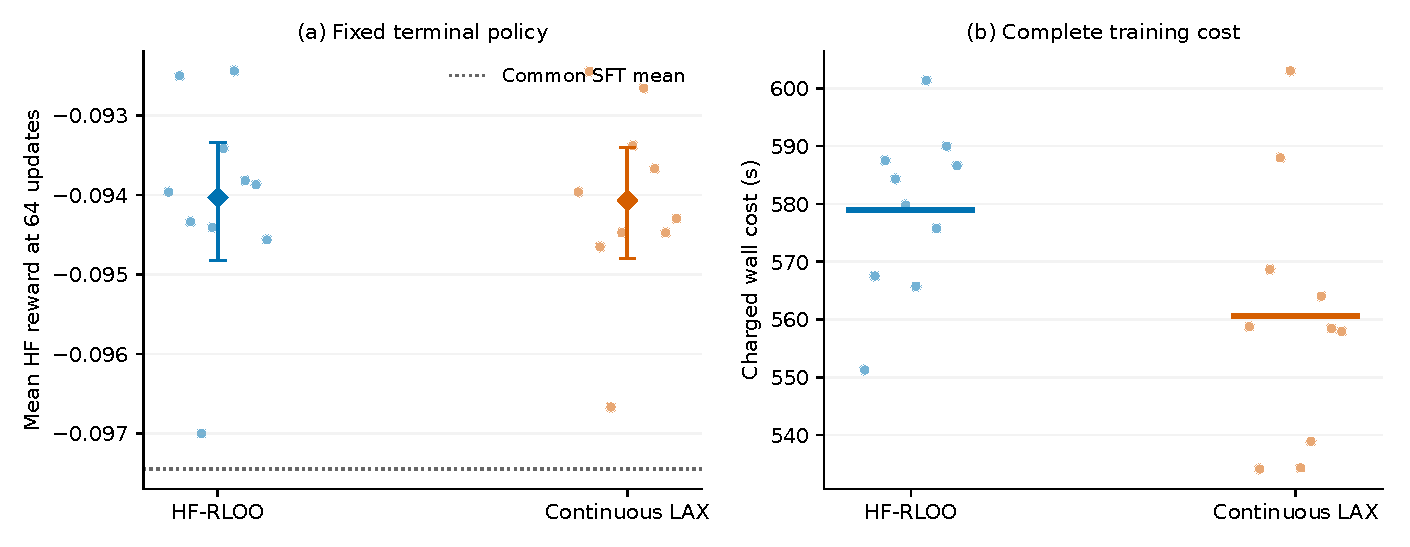
\includegraphics[width=\textwidth]{figures/e5_structured_terminal.pdf}
\caption{Complete structured-policy study at the registered 64-update checkpoint. Dots retain every training seed; diamonds and error bars show means and descriptive 95\% seed-block intervals. The dotted line is the common SFT mean. Right-panel costs include model initialization, actual physical calls, updates, recording and terminal process closure.}
\label{fig:e5-terminal}
\end{figure*}

The predeclared E5 comparison combines the same two recipes across the language and structured policies, retaining all forty trials. Its common charged-cost interval supports an actual matched-cost comparison (Fig.~\ref{fig:e5-frontier}); the original seven-arm study's empty interval is unchanged. The language and structured curves have overlapping descriptive intervals toward the end of this interval. This compares the registered architectures and recipes, including their distinct initialization weights and learning rates; it does not establish a universal preference for a model class. All terminal structured policies have now completed actual deployment, project export and target verification on both public validation contexts. Every first and repeated request is retained, and independent reconstruction from the native high-fidelity state and archived cell volumes confirms the objective components. Cold model and evaluator preparation, complete command costs and warm request costs are recorded separately. The workload calculation includes inference, export and paid verification alongside training. The registered per-task study has also completed all four native optimizers across six tasks and ten seeds. Independent reconstruction verifies every physical call, target-eligible incumbent and complete trial cost. Together with the measured policy deployment, this supplies the reference experiments for the amortization study. The trained policies improve over the registered midpoint rule on both validation contexts for every model seed. Actual language-policy deployment and the quality-matched comparison with the complete optimizers remain the next experiments.

\begin{figure*}[t]
\centering
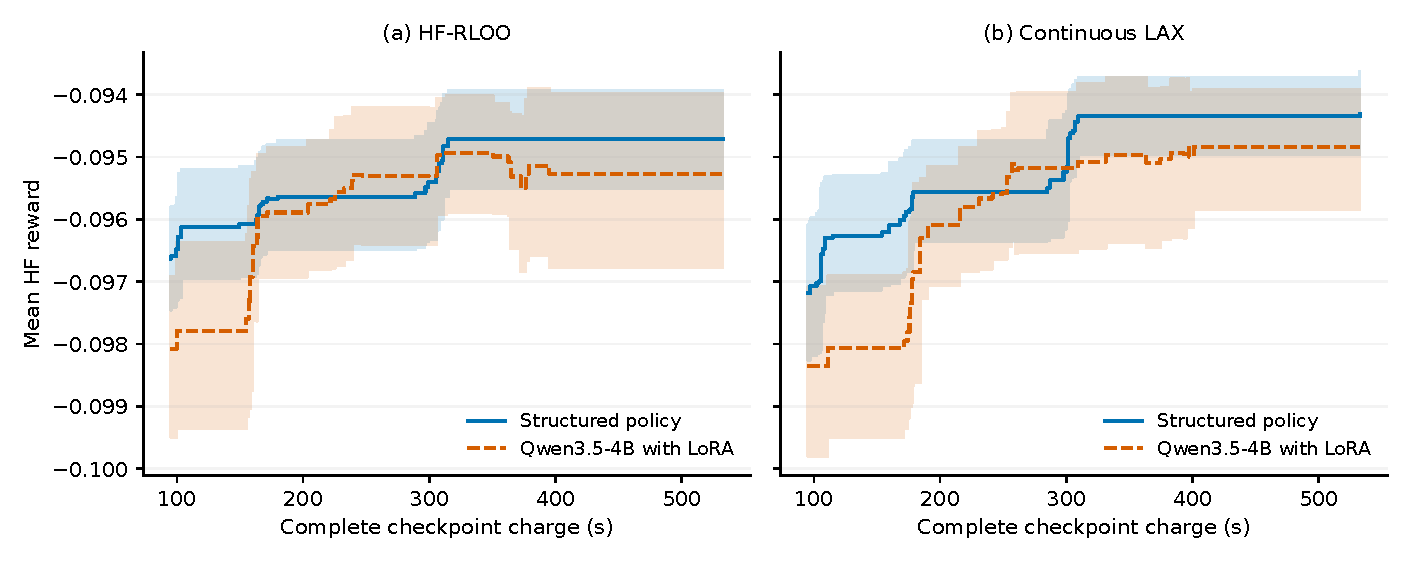
\includegraphics[width=\textwidth]{figures/e5_architecture_frontier.pdf}
\caption{Predeclared E5 comparison on two fixed validation contexts. Each panel uses ten seeds per architecture and the corresponding registered update recipe. The latest affordable checkpoint is evaluated at each charged budget; there is no reward-based checkpoint selection, interpolation or extrapolation. Bands are descriptive pointwise 95\% seed-block mean intervals. Architectures use common requirements and heuristic labels with distinct SFT weights and registered learning rates.}
\label{fig:e5-frontier}
\end{figure*}

The source-explicit original-task MFPG reproduction completes the full seed cohort and supports its improvement over HF-only. Supplementary Material retains its complete curves, native coupling, evaluation isolation and cost evidence. This provides an implementation anchor for the strong-baseline study. The subsequent MFPG-PPO comparison uses the shared physical design objective and the baseline's native surrogate, coupling and allocation mechanism.

\subsection{Flagship and Aerodynamic Evidence}
The Shinaide references establish joint low-fidelity evaluation for the compiled architecture families. All six references are feasible in normal operation and every registered single-unit outage under the synthetic task constraints. Every original context is retained, including the recorded startup failure and its source-only logging repair. Each candidate binds the original server inventory, fan-assisted heat budget and liquid topology to both physical branches. Independent native-state reconstruction agrees with per-server enthalpy closure and the complete device/plant electricity account. The perimeter operators consume actual floor apertures, containment and return paths. Interchangeable equipment and shared mixing nodes explain equal responses in symmetric low-fidelity references. Room-CFD checks will establish the location-dependent higher-fidelity response, and learning studies will measure the design benefit.

The supported aerodynamic benchmark verifies the complete sixteen-dimensional raw drag and lift sensitivities at its registered coarse-grid center. Two-step cold-forward differences and independent native adjoint reconstruction pass the original gates after restoring the wall-distance shape dependence. The derivative bridge preserves the original forward solution and distance algorithm. This closes the local aerodynamic gradient interface needed for the wing study; the registered refined-grid and task-domain experiments supply the remaining evidence.

\subsection{Generalization and Design Automation}
\pending{Held-out requirements and geometries; data-center hard-project validation; second-domain evidence; amortization and deployment cost.}
\section{Discussion}
The completed evidence connects the information interfaces to the design-update mechanism. In the controlled task, target sensitivities and the residual-value control improve the thermal part of the fixed-update comparison. Objective-weighted residual feedback also predicts the target-goal discrepancy more usefully than a raw equation norm on the registered anchors. Together, these observations support information stratification: the useful question is how an available physical signal changes the parameter update relative to its acquisition cost.

The structured-policy comparison shows why both objective decomposition and complete execution costs matter. Its two update recipes reach similar terminal quality while allocating physical calls differently. Thermal improvement and actuator cost can partly offset each other, even when the gradients are correctly connected. The cost--quality study therefore retains the fixed checkpoints, original failures and setup costs, and distinguishes a checkpoint's availability from final process closure. The full controller and strong-baseline experiments will test this allocation mechanism as the policy changes.

The engineering interfaces make the scenario suite executable through source-bound projects and physical records. The six mixed-cooling reference families preserve the original server inventory, fan-assisted heat balance and liquid topology, and support the declared normal and outage contexts. The aerodynamic checks establish the total shape-sensitivity route after restoring the wall-distance dependence. These interfaces provide a coherent foundation for the design-automation experiments. The current inputs retain their declared synthetic provenance and steady heat-generation assumptions; subsequent task-domain and higher-fidelity comparisons use the same explicit acceptance contracts.

\pending{Complete the moving-policy matched-cost comparisons, language-policy deployment, broader task-domain evidence and flagship design study before interpreting the full efficiency and generalization claims.}

\section{Conclusion}
ISPO organizes scalar rewards, physical components, residual feedback and sensitivities within a common budgeted post-training formulation. The verified estimators and controlled learning study support the value of connecting physical information to policy-parameter updates, while the objective-aware correction shows how residual information can be tied to the optimized quantity. Source-bound mixed-cooling and aerodynamic interfaces connect this mechanism to the broader design task suite.
\pending{Add the conclusions of the complete controller, matched-budget baselines, deployment and generalization studies after their registered cohorts and final design checks are complete.}

\bibliographystyle{IEEEtran}
\bibliography{references}
\end{document}
